\problem{}
(a) Figure \ref{fig:p1a} is the histogram image of grain.tif.\\

\begin{figure}[htbp]
    \centering
	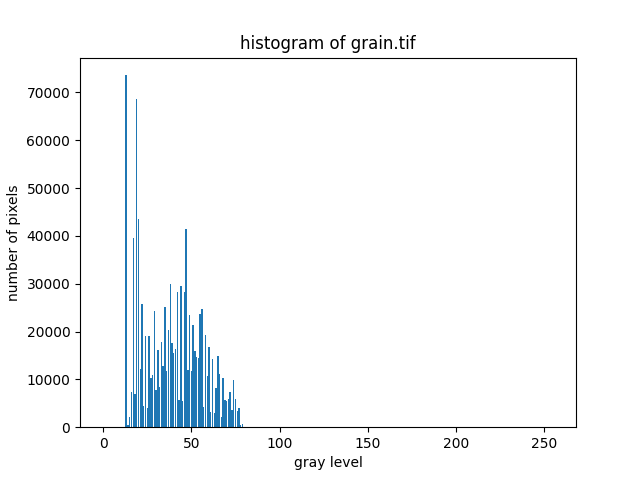
\includegraphics[width=\textwidth]{../images/p1/p1a.png}
    \caption{Histogram of grain.tif}
    \label{fig:p1a}
\end{figure}

(b) The left image of Figure \ref{fig:p1b} is the histogram equalized image, and the right one is 
the histogram of that histogram equalized image.\\

\begin{figure}[htbp]
    \centering
	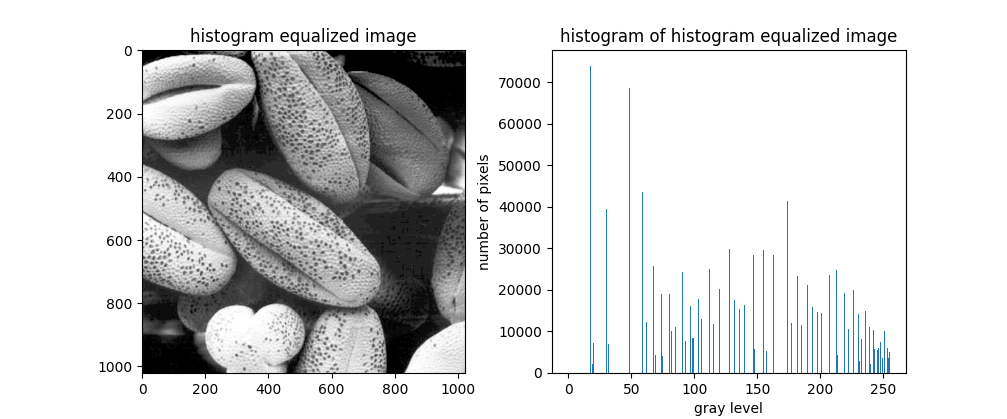
\includegraphics[width=\textwidth]{../images/p1/p1b.png}
    \caption{Histogram equalized image and its histogram}
    \label{fig:p1b}
\end{figure}

(c) The left image of Figure \ref{fig:p1c} is the CLAHE processed image, and the right one is 
the histogram of that CLAHE processed image.\\

\begin{figure}[htbp]
    \centering
	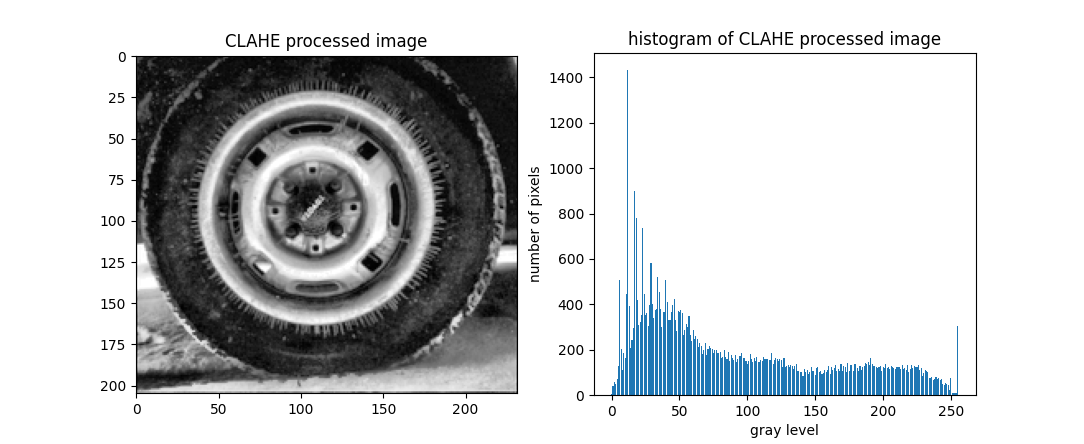
\includegraphics[width=\textwidth]{../images/p1/p1c.png}
    \caption{CLAHE processed image and its histogram}
    \label{fig:p1c}
\end{figure}

\newpage